\documentclass[14pt]{extreport}
\usepackage[utf8]{vietnam}
%\usepackage{type1cm}
\usepackage[left=3.50cm, right=2.00cm, top=3.50cm, bottom=3.00cm]{geometry}
%\usepackage[left=3.0cm, right=1.50cm, top=3.00cm, bottom=2.50cm]{geometry}
\usepackage{graphicx}
\usepackage{mathrsfs} 
\usepackage{amsfonts}
\usepackage{longtable}
\usepackage[intlimits]{amsmath}
\usepackage{array}
\usepackage{amsxtra,amssymb,latexsym,amscd,amsthm}
\usepackage{algorithm}
\usepackage{algorithmic}
\newtheorem{theorem}{\MakeUppercase{K}ết quả}[section]
% khoảng cách dòng 1.5 lines (như trong MS Word)
\renewcommand{\baselinestretch}{1.5}

%——————–
\begin{document}
%tao khung
\newcommand{\Khung}[2]{
\begin{tabular}{|l|}
\hline\rule[-2ex]{0pt}{5.5ex}
\parbox{#1}{#2}\\
\hline
\end{tabular}
}

\Khung{.92\textwidth}{

\begin{center}
\normalsize
\textbf{TRƯỜNG ĐẠI HỌC BÁCH KHOA HÀ NỘI}\\
\normalsize
\textbf{VIỆN TOÁN ỨNG DỤNG VÀ TIN HỌC}\\
\textbf{------------------------------------------------------}\\[0.4cm]

\includegraphics[scale=.2]{logobkdentrang}\\[1.2cm]
\textbf{{\large PHƯƠNG PHÁP PHẦN TỬ HỮU HẠN GIẢI PHƯƠNG TRÌNH STOKES}}\\
\end{center}
\begin{flushleft}
\vspace{1.3cm}
\hspace{1.5cm} \textbf{ Giảng viên hướng dẫn:{ TS. Phan Xuân Thành }}\\[0.2cm]
\hspace{1.5cm} \textbf{ Nhóm Sinh viên thực hiện:}\\[0.2cm]
\hspace{5cm}\textbf{Nguyễn Anh Tú}\\[0.2cm]
\hspace{5cm}\textbf{Phạm Anh Tuấn}\\[0.2cm]
\hspace{1.5cm} \textbf{ Lớp:\hspace{2cm}{ KSTN Toán Tin K60}}\\
\end{flushleft}

\begin{center}
\textbf{{\small HÀ NỘI - 1/2019}}\\
\end{center}
 }
\thispagestyle{empty}
\newpage

\tableofcontents
\newpage

%\listoffigures

\newpage
\chapter{Kiến thức cơ sở}
\section{Tích vô hướng}

$V$- Không gian vectơ trên $R$, tích vô hướng $(u,v)_V: V\times V \rightarrow \mathbb{R}$ có các tính chất: $\forall u,v,w \in V$
\begin{enumerate}
\item $(u,v)=(v,u)$ 
\item $(u,v+w)=(u,v)+(u,w)$
\item $(u, kv) = k(u,v)$
\item $(u,u)\geq 0$
\item $(u,u)=0 \Leftrightarrow  u \equiv \theta  \in V$
\end{enumerate}

Bất đẳng thức:
\begin{align*}
(u,v)^2 \leq (u,u).(v,v) \quad \forall u,v \in V
\end{align*}

\section{Không gian Hilbert}
Không gian vectơ $V$ ($V$ là không gian đủ) với tích vô hướng $(.,.)$ gọi là không gian Hilbert.\\
Chuẩn trong không gian Hilbert:
$$ \left \| u \right \|_V = \sqrt{(u,u)_V}$$\\
Bất đẳng thức của tích vô hướng được chuyển về:
\begin{align*}
|(u,v)| \leq \left \| u \right \|_V.\left \| v \right \|_V
\end{align*}

\section{Đạo hàm yếu}
Xét hàm $u(x), x \in [a,b]$, $u$ khả vi: tồn tại $u'(x)=\underset{h \rightarrow  0}{lim}\frac{u(x+h)-u(x)}{h}$
Đạo hàm yếu của hàm $u(x)$ là hàm $g(x) = \frac{\partial u}{\partial x_k}$ sao cho:
\begin{align*}
\int_{a}^{b}g(x)v(x)dx = - \int_a^bu(x)\frac{\partial v}{\partial x_k}dx  \quad  \forall v \in D(a,b)
\end{align*}
Ta định nghĩa tương tự với đạo hàm cấp $|\alpha|$:
\begin{align*}
D^{\alpha}u = \frac{\partial^{|\alpha|}u }{\partial^{\alpha_1}x_1\partial^{\alpha_2}x_2 ...\partial^{\alpha_n}x_n  }
\end{align*}

\section{Một số không gian hay dùng}
Không gian $L_2(\Omega)$: là không gian các hàm $u(x)$ thoả mãn:
\begin{align*}
\int_{\Omega}\left |  u(x)\right |^{2}dx < +\infty 
\end{align*}
Chuẩn và tích vô hướng cho không gian $L_2(\Omega)$:
\begin{align*}
\left \| u \right \|_{L_2(\Omega)} &= \left ( \int_{\Omega}\left |  u\right |^{2}dx \right )^{\frac{1}{2}}\\
(u,v)_{L_2(\Omega)} &= \int_{\Omega}u(x)v(x)dx
\end{align*}
Do không gian $L_2(\Omega)$ là không gian Hilbert nên:
\begin{align*}
\left ( \int_{\Omega}u(x)v(x)dx \right )^2 &\leq \int_{\Omega}\left |  u\right |^{2}dx. \int_{\Omega}\left |  v\right |^{2}dx
\end{align*}
Tương tự cho không gian $L_p(\Omega)$: là không gian các hàm $u(x)$ thoả mãn $\int_{\Omega}\left |  u\right |^{p}dx < +\infty $
\begin{align*}
\left \| u \right \|_{L_p(\Omega)} &= \left ( \int_{\Omega}\left |  u\right |^{p}dx \right )^{\frac{1}{p}}\\
\left | \int_{\Omega}u(x)v(x)dx \right | &\leq \left ( \int_{\Omega}\left |  u\right |^{p}dx \right )^{\frac{1}{p}}.\left ( \int_{\Omega}\left |  v\right |^{q}dx \right )^{\frac{1}{q}}
\end{align*}
với $\frac{1}{p}+\frac{1}{q}=1$\\
Không gian $W_p^m(\Omega)$:  $H^m(\Omega) \equiv  W^m_2(\Omega)$
\begin{align*}
W_m^p(\Omega) = \{ u | D^{\alpha}u \in L_p(\Omega) \forall \alpha : |\alpha|\leq m, m \in \mathbb{N}\}
\end{align*}

Chuẩn và tích vô hướng:
\begin{align*}
(u,v)_{H^m(\Omega)} &= \sum_{|\alpha|\leq m}(D^{\alpha}u, D^{\alpha}v)_{L_2(\Omega)}\\
(u,v)_{L_2(\Omega)} &= \int_{\Omega}u(x)v(x)dx\\
\left \|  u\right \|_{H^m(\Omega)} &= \sqrt{(u,u)_{H^m(\Omega)}}
\end{align*}

Không gian $H^m(\Omega)$: là không gian Hilbert: $H^0(\Omega) \equiv  L_2(\Omega)$:
\begin{align*}
\left \| u \right \|_{H^1(\Omega)}= \sqrt{\int_{\Omega}u^2(x)dx+\sum_{k=1}^n\int_{\Omega}\left ( \frac{\partial u}{\partial x_k} \right )^2dx}
\end{align*}


\section{Bất đẳng thức Poincare}
Xét $\Omega \subset \mathbb{R}^n$, $\Omega$ bị chặn. Với $\forall  u \in H^1(\Omega)$, tồn tại hằng số $C$ (phụ thuộc $\Omega$) sao cho:
\begin{align*}
\int_{\Omega}u^2(x)dx \leq C\left (  \sum_{k=1}^{n}\int_{\Omega}u_{x_k}^{2}dx+\oint_{\Gamma}u^{2}(x)dS\right )
\end{align*}

Trong các phần sau, để cho ngắn gọn, khi miền xác định đã rõ, ta kí hiệu
$$||u||_0 := ||u||_{L_2(\Omega)}$$
$$||u||_1 := ||u||_{H_1^0(\Omega)}$$

\chapter{Hệ phương trình Stokes}
{\normalsize
Trong bài báo cáo này, chúng ta quan tâm đến việc giải gần đúng nghiệm của hệ phương trình Stokes đối với bài toán dòng chảy không nhớt. Ở dạng đơn giản nhất, hệ phương trình Stokes trong trường hợp 2 chiều trên miền $\Omega$ được phát biểu như sau:
$$
\begin{cases}
-\Delta u + grad p \ = \ f \\
div u = 0 \\
u|_{\Gamma} = g
\end{cases}
$$
trong đó $u$ là hàm vector khả vi hai lần trên miền $\Omega$ và $\Gamma = \partial \Omega$
\section{Xây dựng bài toàn yếu}
Đặt $e_{ij}(u) =  \frac{1}{2} ( \frac{\partial u_i}{\partial x_j} + \frac{\partial u_j}{\partial x_i})$ $\forall i,j = 1,2$. Ta có
\begin{equation} \label{eq1}
\begin{split}
\sum_{j=1}^{2} \frac{\partial}{\partial x_j} e_{kj}(u) & = \sum_{j-1}^2 \frac{1}{2} \left(\frac{\partial^2 u_k}{\partial x_j^2} + \frac{\partial^2 u_j}{\partial x_j \partial x_k}\right) \\
 & = \frac{1}{2} \sum_{j=1}^2 \frac{\partial^2 u_k}{\partial x_j^2} + \frac{1}{2} \sum_{j=2}^2 \frac{\partial^2 u_j}{\partial x_j \partial x_k} \\
 & = \frac{1}{2} \sum_{j=1}^2 \frac{\partial^2 u_k}{\partial x_j^2} + \frac{1}{2} \frac{\partial}{\partial x_k} \left(\sum_{j=1}^2 \frac{\partial u_j}{\partial x_j} \right) \\
 & = \frac{1}{2} \Delta u_k(x) + \frac{1}{2} \frac{\partial}{\partial x_k} div \ u(x) \ \ \forall \ k = 1,2
\end{split}
\end{equation}
Nhân thêm hàm thử $v_k(x)$
\begin{equation} \label{eq2}
\begin{split}
\sum_{j=1}^{2} \frac{\partial}{\partial x_j} e_{kj}(u) v_k(x) & = v_k(x) \sum_{j=1}^2 \frac{\partial}{\partial x_j} e_{kj} (u) + \sum_{j=1}^2 e_{kj}(u) \frac{\partial v_k(x)}{\partial x_j} \\
 & = \frac{1}{2} v_k(x) \Delta u_k + \frac{1}{2} v_k \frac{\partial}{\partial x_k} div u(x) + \sum_{j=1}^2 e_{kj}(u) \frac{\partial v_k(x)}{\partial x_j}
\end{split}
\end{equation}
Lấy tổng trên $k = 1,2$ ta có
\begin{equation} \label{eq3}
\begin{split}
\sum_{k,j=1}^{2} \frac{\partial}{\partial x_j} e_{kj}(u) v_k(x) & = \frac{1}{2} \sum_{k=1}^2 \left[ \Delta u_k + \frac{\partial}{\partial x_k} div \ u(x) \right] v_k(x) + \sum_{i, j=1}^2 e_{kj}(u) e_{kj}(v)
\end{split}
\end{equation}
Chuyển $\Delta u_k$ sang vế trái, ta thu được
\begin{equation} \label{eq4}
\begin{split}
- \sum_{k=1}^2 v_k(x) \Delta u_k(x) & = 2 \sum_{k,j=1}^2 e_{kj}(u) e_kj(v) - 2\sum_{i,j=1}^2 \frac{\partial}{\partial x_j} (e_{kj}(u) v_k(x)) \\
& + \sum_{k=1}^2 v_k(x) \frac{\partial}{\partial x_k} div \ u(x)
\end{split}
\end{equation}

Nhân hai vế của phương trình Stoke $- \Delta u + \nabla p(x) = f(x)$ với hàm thử $v(x)$ và lấy tích phân trên miền $\Omega$, ta có
\begin{equation} \label{eq5}
\begin{split}
\int_{\Omega} f_k(x) v_k(x) dx & = - \int_{\Omega} v_k(x) \Delta u_k(x) dx + \int_{\Omega} \frac{\partial p(x)}{\partial x_k} v_k(x) dx \\
 & = - \int_{\Omega} v_k(x) \Delta u_k(x) dx - \int_{\Omega} p(x) \frac{\partial v_k}{\partial x_k} dx + \int_{\Gamma} p(x) v_k(x) n_k(x) dS  \\
& \forall k = 1,2
\end{split}
\end{equation}

Lấy tổng theo $k = 1,2$, và thay vào phương trình $(4)$, ta thu được
\begin{equation} \label{eq6}
\begin{split}
\int_{\Omega} v(x)^T f(x) dx & = 2 \sum_{k, j = 1}^2 \int_{\Omega} e_kj(u, x) e_{kj} (v,x) - 2 \sum_{k,j=1}^2 \int_{\Omega} \frac{\partial}{\partial x_j} \left[ e_{kj}(u, x) v_k(x) \right] \\
& + \sum_{k=1}^2 \int_{\Omega} v_k(x) \frac{\partial}{\partial x_k} div \ u(x) dx - \int_{\Omega} p(x) div \ v(x) dx \\
& + \sum_{k =1}^2 \int_{\Gamma} v_k(x) n_k(x) dS 
\end{split}
\end{equation}

Áp dụng công thức tích phân từng phần ta thu được công thức Green cho bài toán Stoke
\begin{equation} \label{eq7}
\begin{split}
\int_{\Omega} v(x)^T f(x) dx & = 2 \sum_{k, j = 1}^2 \int_{\Omega} e_kj(u, x) e_{kj} (v,x) + 2 \sum_{k,j=1}^2 \int_{\Gamma} e_{kj}(u, x) v_k(x) n_j(x) dS \\
& - \int_{\Omega} div \ u div \ v dx + \int_{\Gamma} div \ u n^T(x) v(x) dS \\
& - \int_{\Omega} p(x) div \ v dx + \sum_{k =1}^2 \int_{\Gamma} p(x) v_k(x) n_k(x) dS 
\end{split}
\end{equation}

Chọn hàm thử $v \in [ H_0^1(\Omega) ]^2$, vì $u$ bằng 0 trên biên $\Gamma$ và $div \ u = 0$, nên ta có

\begin{equation} \label{eq8}
\begin{split}
2 \sum_{k,j = 1}^2 \int_{\Omega} e_{kj}(u,x) e_{kj} (v,x) dx - \int_{\Omega} p div \ v dx = \int_{\Omega} v^T(x) f(x) dx \ \forall \ v \in [ H_0^1(\Omega) ]^2
\end{split}
\end{equation}

Đặt :
$$\alpha(u, v) = 2 \sum_{k,j = 1}^2 \int_{\Omega} e_{kj}(u,x) e_{kj} (v,x)$$
$$\beta(v, q) = \int_{\Omega} q(x) \ div \ v dx$$
Ta thấy rằng nghiệm của $p(x)$ có thể sai khác nhau một hằng số, do đó đặt $Q = {q(x) |in L_2(\Omega) \ và \ \int_{\Omega} q(x) dx = 0 }$. Ta có bài toán yếu cho phương trình Stoke: \\
Tìm hàm $u \in  [ H_0^1(\Omega) ]^2$ và hàm $p \in Q$ sao cho
$$
\begin{cases}
\alpha(u,v) - \beta(v, p) = <f, v> \ \forall \ v \in [ H_0^1(\Omega) ]^2 \\
\beta(u, q) = 0 \ \forall \ q \in Q
\end{cases}
$$

\section{Tính đặt chỉnh}
Ở dạng tổng quát, bài toán Stoke được gọi là bài toán hỗn hợp (mixed problem) được miêu tả như sau [4]:
\begin{center}
Tìm $u \in V$  và $p \in M'$  thỏa mãn
\end{center}
$$
\begin{cases}
Au + B^*p = f, \\
Bu = g
\end{cases}
$$
trong đó $V$ và $M$ là hai không gian Banach, $A: V \rightarrow V'$ và $B: V \rightarrow M$ là hai ánh xạ tuyến tinh bị chặn (ở đây, ta kí hiệu $X'$ là không gian đối ngẫu của $X$). $B*: M' \rightarrow V'$ là toán tử đối ngẫu của $B$ (adjoint operator), $f \in V'$ và $g \in M$. Mục đích của phần này là ta sẽ miêu tả tính đặt chỉnh (well-posedness) của hệ phương trình trên, từ đó liên hệ với bài toán Stoke. \\

Gọi $ker(B)$ là nhân của toán tử $B$ và $A_{\pi}: ker(B) \rightarrow ker(B')$ sao cho $<A_{\pi}v, w>_{V', V} = <Av, w>_{V', V}$ với mọi $v, w \in ker(B)$, khi đó $A_{\pi} = J_B^*AJ_B$ với $J_B$ là đơn ánh từ $ker(B)$ vào $V$ và $J_B^*$ là toán tử đối ngẫu của $J_B$. Theo [4], ta có định lý sau về tính đặt chỉnh của phương trình trên
\begin{theorem}
Phương trình trên là đặt chỉnh khi và chỉ khi $A_{\pi}$ là đẳng cấu và $B$ là toán ánh
\end{theorem}

Giả sử rằng, $V$ và $M$ là không gian Banach phản xạ (reflexive Banach) và $Q = M'$. Bây giờ, ta xét hai dạng song tuyết tính bị chặn $\alpha(V, V)$ và $\beta(V, Q)$, thỏa mãn $\alpha(v, w) =  <Av, w>_{V', V}$ và $b(v, q) = <Bv, q>_{Q', Q}$. Đặt
\begin{equation} \label{eq8}
\begin{split}
||\alpha|| & = \sup_{(v, w) \in V x V} \frac{\alpha(v,w)}{||v||_V||w||_V} \\
||\beta|| & = \sup_{(v, q) \in V x Q} \frac{\beta(v,q)}{||v||_V||q||_Q}
\end{split}
\end{equation}
Với $f \in V'$ và $g \in Q'$. Hệ phương trình có thể viết lại như sau:
\begin{center}
Tìm $u \in V$  và $p \in Q$  thỏa mãn
\end{center}
$$
\begin{cases}
\alpha(u, w) + \beta(w,p) = f(w), \ \forall w \in V \\
\beta(u,q) = g(q), \ \forall q \in Q
\end{cases}
$$
Ở đây, ta kí hiệu $f(v) = <f, v>_{V', V}$ và $g(q) = <g,q>_{Q', Q}$.
Khi đó, ta có định lý sau về tính đặt chỉnh
\begin{theorem}
Hệ phương trình trên đặt chỉnh (well-posed) khi và chỉ khi
\begin{equation} \label{eq8}
\begin{split}
\inf_{v \in ker(B)} \sup_{w \in ker(B)} \frac{\alpha(v,w)}{||v||_V||w||_V} = a > 0 \\
\inf_{q \in Q} \sup_{v \in V} \frac{\beta(v, q)}{||v||_V||q||_Q} = b > 0
\end{split}
\end{equation}
\begin{center}
và $\forall w \in ker(B)$, nếu $\alpha(v, w) = 0$ với mọi $v \in ker(B)$ thì w = 0
\end{center}
\end{theorem}

Ở đây, ta thấy rằng, nếu $\alpha(u, v)$ là $V-elliptic$ thì khí đó điều kiện thứ nhất và điều kiện thứ ba dễ dàng được thỏa mãn
\chapter{Phương trình Stoke bằng phương pháp phần tử hữu hạn}
\section{Phần tử hữu hạn cho bài toán Stoke}
Trong phần này, ta đi giải bài toán yếu của phương trình stoke bằng phương pháp phần tử hữu hạn, tức là ta đi tìm hàm $u_h$, $v_h$ thuộc vào hai không gian con hữu hạn chiều $V_h$, $Q_h$ của $[ H_0^1(\Omega) ]^2$ và $L_2(\Omega)$ thỏa mãn phương trình
$$
\begin{cases}
\alpha(u_h,v) - \beta(v, p_h) = <f, v> \ \forall \ v \in V_h \\
\beta(u_h, q) = 0 \ \forall \ q \in Q_h
\end{cases}
$$

Theo [1], ta cần phải chọn không gian $V_h$ và $Q_h$ thỏa mãn điều kiện inf-sup
$$\inf_{q_h \in Q_h} \sup_{v_h \in V_h} \frac{\int_{\Omega} q_h \ div \ v_h dx}{||v_h||_{1} ||q_h||_{0/R}}$$

Trong phần này, bài báo cáo sẽ chỉ ra một cách xây dựng hai không gian thỏa mãn điều kiện inf-sup. Ta biết răng, bài toán Stoke thỏa mãn điều kiện inf-sup, theo [2], để kiêm tra điều kiện inf-sup cho hai không gian con hữu hạn chiều $V_h$ và $Q_h$ ta cần xây dựng một ánh xạ $\Pi_h : [H_0^1 (\Omega)]^2 \rightarrow V_h$ sao cho
$$
\begin{cases}
\int_{\Omega} q_h div(\Pi_hv - v) dx = 0 \\
||\Pi_hv|| \leq c ||v||
\end{cases}
$$
Vì $q_h$ có khả vi cấp một, sử dụng công thức tích phân từng phần, ta có điều kiện đầu tương đương với
\begin{equation} \label{eq9}
\begin{split}
\int_{\Omega} (v - \Pi_hv) grad \ q_h dx = 0 \ \forall \ q_h \ \in Q_h
\end{split}
\end{equation}

Ở đây, miền $\Omega$ là một miền đa giác trong không gian hai chiều và được chia thành các phần tử hữu hạn là các tam giác $T$. Và nếu $q_h$ là hàm đa thức bâc $k$ trên mỗi tam giác $T$, điều kiện (9) tương đương với
\begin{equation} \label{eq10}
\begin{split}
\int_{T} (v - \Pi_hv) \Phi_h dx = 0 \ \forall \ \Phi_h \ \in P_{k-1}(T)
\end{split}
\end{equation}
Gọi một cách chia miền $\Omega$ thành các phần tử hữu hạn là $T_h$. Ta định nghĩa
$$M^k(T_h) \ \{ v| v\in C^0(\Omega), v_{|T} \in P_k(T) \ \forall T \in T_h \}$$
$$M_0^k(T_h) = M_0^k(T_h) \cap H_0^1(\Omega)$$
$$B^k(T_h) = \{ v | v_{|T} \in P_k(T) \cap H_0^1(T) \ \forall T \in T_h \}$$

Phương pháp phần tử hữu hạn MINI sử dụng không gian
$$V_h = (M_0^1)^2 \bigoplus (B^3)^2$$
$$Q_h = M_0^1$$

Trong trường hợp này, điều kiện (10) trở thành
\begin{equation} \label{eq11}
\begin{split}
\int_T (v - \Pi_hv) dx = 0 \ \forall \ T, \ \forall \ v \in (H_0^1)^2
\end{split}
\end{equation}

Với cách chọn không gian như trên, ta chỉ cần xây dựng ánh xạ $\Pi_h$ thỏa mãn điều kiện được miêu tả như trên (theo [2]) để chứng minh rằng cách chọn không gian như vậy thỏa mãn điều kiện inf-sup. Theo [3], ta có thể xây dựng được ánh xạ $\overline{\Pi}_h: (H_0^1)^2 \rightarrow (M_0^1)^2$ thỏa mãn (với $r = 0,1$ và $h_T = diam T$)
\begin{equation} \label{eq12}
\begin{split}
\sum_T h_T^{2r-2} ||\overline{\Pi}_hv - v||_{r, T}^2 \leq C ||v||_{1, \Omega}^2
\end{split}
\end{equation}
Để đảm bảo điểu kiện (11), ta cộng thêm vào ánh xạ $\overline{\Pi}_h$ một bội số của hàm bubble trên mỗi tam giác. Cụ thể, ta đặt
\begin{equation} \label{eq13}
\begin{split}
\Pi_hv = \overline{\Pi}_hv + \alpha_T \Phi_T
\end{split}
\end{equation}

Để thỏa mãn điều kiện (11), ta có
\begin{equation} \label{eq14}
\begin{split}
\alpha_T \int_T \Phi_T dx = \int_T (\overline{\Pi}_hv - v)dx
\end{split}
\end{equation}

Ta có
\begin{equation} \label{eq15}
\begin{split}
||\Pi_hv||_{1, T} \leq ||\overline{\Pi}_h||_{1, T} + ||\alpha_T \Phi_T||_{1, T}
\end{split}
\end{equation}

Mặt khác, ta có
\begin{equation} \label{eq16}
\begin{split}
||\alpha_T \Phi_T|| & \leq c ||\alpha_T||\\
|\alpha_T| & \leq ch_T^{-1} ||\Pi_hv - v||_{0, T}
\end{split}
\end{equation}

Lấy tổng theo $T$ và sử dụng (12) ta chứng minh được phương phần tử MINI thỏa mãn điều kiện inf-sup. \\
Trên mỗi tam giác $T$, hàm $u$ và $p$ được xấp xỉ bằng tổ hớp tuyến tính của các hàm cơ sở như sau
\begin{equation} \label{eq17}
\begin{split}
u(\mathbf{x}) = \sum_{i=1}^3 \phi_i(\mathbf{x}) u_i + \phi_b(\mathbf{x}) u_b \\
p(\mathbf{x}) = \sum_{i=1}^3 \phi_i(\mathbf{x})p_i
\end{split}
\end{equation}
trong đó $u_i$ vàn $p_i$ là giá trị nốt của hàm u $u$ và $p$. Phương pháp phần tử hữu hạn $P^1-bubbble / P^1$(MINI) sử dụng hàm các hàm cở được định nghĩa như sau
$$\Phi_1(\mathbf{x}) = 1 - x-y, \ \Phi_2(\mathbf{x}) = x, \ \Phi_3(\mathbf{x}) = y, \ \Phi_b(\mathbf{x}) = 27 \Phi_1(\mathbf{x})\Phi_2(\mathbf{x})\Phi_3(\mathbf{x})$$

Nếu ta đặt
\[
\overline{u}_i
=
\begin{bmatrix}
    u_1^i \\
    u_2^i \\
    u_{i, b}
\end{bmatrix}
, i = 1,2
\]

\[
\overline{f}_i
=
\begin{bmatrix}
    f_1^i \\
    f_2^i \\
    f_{i, b}
\end{bmatrix}
, i = 1,2
\]
Thì hệ phương trình Stoke trên một phần tử hữu hạn có thể viết được dưới dạng như sau,
\begin{equation}
  \begin{bmatrix}
    \overline{A} & 0 & -\overline{B}_1^t \\
    0 & \overline{A} & -\overline{B}_2^t \\
    -\overline{B}_1 & -\overline{B}_2 & 0
  \end{bmatrix}
  \begin{bmatrix}
    \overline{u}_1 \\
    \overline{u}_2 \\
    p
  \end{bmatrix}
  =
  \begin{bmatrix}
    \overline{f}_1 \\
    \overline{f}_2 \\
    0
  \end{bmatrix}
  \label{eq18}
\end{equation}
trong đó
\begin{equation} \label{eq19}
\begin{split}
\overline{A}^T_{ij} & = \int_T \nabla \Phi_i . \nabla \Phi_j dx \\
\overline{B}^T_{ij} & = \int_T \partial_1 \Phi_i \Phi_j dx + \int_T \partial_2 \Phi_i \Phi_j dx \\
\overline{f}^T_i & = \int_T f \Phi_i dx
\end{split}
\end{equation}
Ta cần phải ghép và tính toán các phần tử của ma trận để thu được hệ phương trình trên toàn bộ miền $\Omega$
\section{Các phần tử trên ma trận}
Để giải quyết bài toán, ta chia miền chữ nhật như sau
\begin{center}
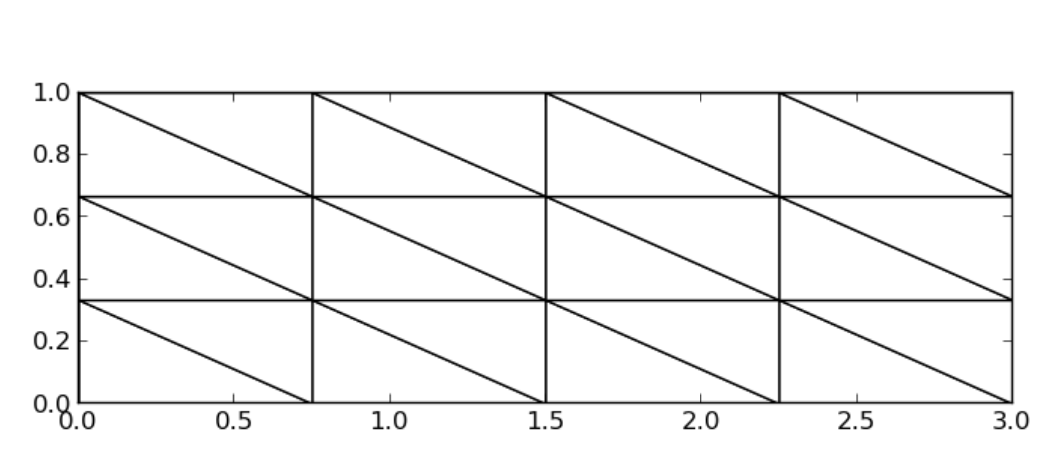
\includegraphics[scale=0.5]{grid_fem.PNG}
\end{center}
Với mỗi tam giác $T$, gọi $\{ (x_i, y_i) \}_{i = 1,2,3}$ là các đỉnh và $\{ \Phi_i \}_{i =1,2,3}$ là các hàm cơ sở tương ứng. Khi đó, gradient của $\Phi_i$ được tính bằng công thức sau
\begin{equation} \label{eq20}
\begin{split}
  \begin{bmatrix}
    \nabla \Phi_1^t \\
    \nabla \Phi_2^t \\
	\nabla \Phi_3^t
  \end{bmatrix}
  =
  \frac{1}{2 |T|}
  \begin{bmatrix}
    y_2 - y_3 & x_3 - x_2 \\
    y_3 - y_1 & x_1 - x_3 \\
    y_1 - y_2 & x_2 - x_1
  \end{bmatrix}
\end{split}
\end{equation}
với $|T|$ là diện tích của tam giác $T$, được tính bằng công thức
\begin{equation} \label{eq21}
\begin{split}
2 |T| = det
\begin{bmatrix}
    x_2 - y_1 & x_3 - x_1 \\
    y_2 - y_1 & y_3 - y_1 \\
  \end{bmatrix}
\end{split}
\end{equation}

Ta kí hiệu
$$x_{ij} = x_i - x_j, \ y_{ij} = y_i - y_j$$
và
\[
x^{(T)}
=
\begin{bmatrix}
    x_{32} \\
    x_{13} \\
    x_{21}
\end{bmatrix}
\]

\[
y^{(T)}
=
\begin{bmatrix}
    y_{23} \\
    y_{31} \\
    y_{12}
\end{bmatrix}
\]

Lí do đưa ra hai vector $x^{(T)}$ và $y^{(T)}$ vì nó sẽ được sử dụng để thực hiện lập trình song song trong chương trình Matlab. Khi đó các phần tử của ma trận $\overline{A}$ được tính như sau
\begin{equation} \label{eq22}
\begin{split}
\overline{A}_{ij} = \int_T \nabla \Phi_i \nabla \Phi_j dx = \frac{1}{4|T|} (y_i^{(T)} y_j^{(T)} + x_i^{(T)} x_j^{(T)})
\end{split}
\end{equation}
Khi đó, các phần tử không chứa bubble của ma trận $A$ có thể tính như sau:
$A = \frac{1}{4|T|} \left[ y^{(T)}(y^{(T)})^t + x^{(T)}(x^{(T)})^t \right]$

Vì $\overline{A}$ là ma trận đối xứng, nên ta chỉ cần còn phải tính $\overline{bj}$ với $j = 1,2,3,b$.
\begin{equation} \label{eq23}
\begin{split}
\overline{A}_{bj} =\frac{9|T|}{4} \sum_{i=1}^3 \nabla \Phi_i = 0, \ j =1,2,3
\end{split}
\end{equation}

\begin{equation} \label{eq24}
\begin{split}
\overline{A}_{bb} & = \int_T 27^2 \nabla(\Phi_1 \Phi_2 \Phi_3) \nabla(\Phi_1 \Phi_2 \Phi_3) dx \\
& = \frac{81 |T|}{10} (|\nabla \Phi_1|^2 + |\nabla \Phi_1|^2 + |\nabla \Phi_1|^2 + \nabla \Phi_1\nabla \Phi_2 + \nabla \Phi_2\nabla \Phi_3 + \nabla \Phi_1\nabla \Phi_3) \\
& =: \omega_A
\end{split}
\end{equation}
Như vậy, với kết quả trên, ma trận $\overline{A}$ có dạng
\[
\overline{A} = 
\begin{bmatrix}
A & 0 \\
0 & \omega_A
\end{bmatrix}
\]

Bây giờ, ta đi tính các phần tử của ma trận $\overline{B}_i$. Ta có
\begin{equation} \label{eq25}
\begin{split}
-(\nabla u_h, q_h) & = \overline{B} = \left[ -\overline{B}_1 - \overline{B}_2 \right] \\
& = |T| 
\begin{bmatrix}
-s \nabla \Phi_1 & -s \nabla \Phi_2 & -s \nabla \Phi_3 & t \nabla \Phi_1 \\
-s \nabla \Phi_1 & -s \nabla \Phi_2 & -s \nabla \Phi_3 & t \nabla \Phi_2 \\
-s \nabla \Phi_1 & -s \nabla \Phi_2 & -s \nabla \Phi_3 & t \nabla \Phi_3
\end{bmatrix}
\end{split}
\end{equation}
Trong đó $s = \frac{1}{3}$ và $t = \frac{9}{20}$. Khi đó ta đặt
\[
B_i = \frac{|T|}{3}
\begin{bmatrix}
\partial_i \Phi_1 & \partial_i \Phi_2 & \partial_i \Phi_3 \\
\partial_i \Phi_1 & \partial_i \Phi_2 & \partial_i \Phi_3 \\
\partial_i \Phi_1 & \partial_i \Phi_2 & \partial_i \Phi_3 
\end{bmatrix}
\]
\[
B_{ib} = \frac{9|T|}{20}
\begin{bmatrix}
\partial_i \Phi_1 \\
\partial_i \Phi_2 \\
\partial_i \Phi_3
\end{bmatrix}
\]
Khi đó, ta có
$$\overline{B}_i = |B_i - B_{ib}|$$
và
\begin{equation} \label{eq26}
\begin{split}
B_{1ij} = \frac{|T|}{3} \partial_1 \Phi_i
\end{split}
\end{equation}
Sử dụng các kết quả trên, các phần tử của ma trận $B_1$ và $B_2$ trở thành
\[
B_1 = \frac{1}{6}
\begin{bmatrix}
(y^{(T)})^t \\
(y^{(T)})^t \\
(y^{(T)})^t
\end{bmatrix}
\]
\[
B_2 = \frac{1}{6}
\begin{bmatrix}
(x^{(T)})^t \\
(x^{(T)})^t \\
(x^{(T)})^t
\end{bmatrix}
\]
$$B_{1b} = \frac{9}{40} y^{(T)}, \ $$

Cuối cùng ta chỉ còn phải tính các phần tử của ma trận vế phải. Cụ thể, ta có
\begin{equation} \label{eq27}
\begin{split}
f_i^{(T)} = \frac{|T|}{3} f_{iT}
\begin{bmatrix}
1 \\
1 \\
1
\end{bmatrix}
\end{split}
\end{equation}
trong đó $f_{iT}$ là giá trị trung bình của hàm $f_i$ trên tam giác $T$
$$f_{iT} = (f_i(x_1) + f_i(x_2) + f_i(x_3))$$

\chapter{Kết quả}

\end{document}
